\chapter{تنظیمات سندباکس و میزبان}
\section{اتصال به 
    \lr{\lr{127.0.0.1}}
     با نامی دیگر}
ددر فصل گذشته (اول) این کتاب به بررسی برخی مفاهیم و نحوه نصب و ایجاد یک ماشین مجازی در نرم‌افزار ویرچوال‌باکس پرداختیم. در این فصل قصد داریم تا به نحو تنظیم اس‌اس‌اچ «SSH» برای سیستم میزبان جهت دسترسی به سیستم مهمان و سپس تنطیم آپاچی و تنظیم این کارساز وب متن‌باز بپردازیم.در فصل سوم این آموزش نیز با نصب مای‌اس‌کی‌یو‌ال و PHP به معرفی و اجرای چند برنامه کوچک و تنظیم و تست آنان خواهیم پرداخت.

بعد از انجام آموزش فصل اول، حال ما دارای یک سیستم‌عامل سرور هستیم که دارای نرم‌افزارهای پایه‌ای برای اجرای یک سرور محلی هستیم. برای مدیریت و پیکربندی این سرور نیاز به برخی تنظیمات و تغییرات نیز هست تا بتوانیم از این سرور استفاده کنیم. کارسازهای وب محلی در ابتدا نیاز به کمی تغییرات و تنظیمات دارند، مخصوصا اگر در ویرچوال‌باکس نصب شده باشند که علاوه بر کارهای عادی باید برخی تنظیمات را نیز انجام دهیم. تنظیمات مورد نیاز برای اجرای اوبونتو مخصوص کارساز وب را در ویرچوال‌باکس و ماشین مجازی مورد نظر، تنظیم کرده‌ایم. اما در خود اوبونتو سرور نیاز به نصب راه‌انداز و استفاده از آن داریم. علاوه بر نصب گرداننده و راه‌اندازهای مورد نیاز برای استفاده در اوبونتو ابتدا باید بتوانیم از طریق سیستم خود و یا حتی از راه دور، به خط فرمان سیستم‌عامل ماشین مهمان دسترسی داشته باشیم. برای این‌کار باید از SSH استفاده کنیم.

به دلیل آنکه ممکن است شما یک توسعه‌دهنده وب باشید و در برخی مواقع ممکن است سیستم‌عامل مورد استفاده شما گنو/لینوکس نباشد و از مک یا ویندوز استفاده کنید، طریقه نصب و تنظیم اس‌اس‌اچ را در سیستم‌عامل‌های او‌اس‌ ده و ویندوز نیز آموزش خواهیم داد به هر حال ذهنیت پیش‌فرض برای ما این موضوع است که شما کاربر گنو/لینوکس هستید، اما استفاده از این آموزش در ماشین‌مجازی برای نصب اوبونتو و پیکربندی LAMP تقریبا در هر سیستم‌عاملی که ویرچوال‌باکس در آن نصب شود نیز قابل انجام است. بنابراین اگر کاربر ویندوز و مک هم هستید، هرگز نباید نگران این موضوع باشید، زیرا ما هر دو سیستم‌عامل بالا را نیز در این آموزش پوشش داده‌ایم. سیستم‌عامل او‌اس ۱۰ هم که در اکثر نکات همانند گنو/لینوکس است.

در این‌جا ما برخی تنظیمات را به گونه‌ای در نظر می‌گیریم که شما در استفاده از سندباکس راحت باشید و نیازی به وارد کردن رمز عبور و … در هر مرتبه و هر بار ورود نباشید، همچنین دیگر تنظیمات برای راحتی کار شما در استفاده از سندباکس است.  با وجود این تمامی موارد بالا، فقط در سندباکس عقلانی است و برای یک سرور واقعی توصیه نمی‌شود که چنین کارهایی انجام شود.  بنا بر این در هر آموزش کاملا تاکید می‌شود که این کار را فقط در سندباکس توصیه می‌کنیم  که در سرور واقعی چنین تنظیماتی را اعمال نکنید، زیرا ممکن است امنیت سرور شما را به خطر بیندازند.

\section{سیستم‌عامل گنو/لینوکس و اواس ده،}

برای اتصال به یک سرور معمولا ما به یک آدرس و یا یک آی‌پی «IP» نیاز داریم. آی‌پی یک میزبان محلی همواره 
\url{\lr{127.0.0.1}}
 است که با نام 
 \url{«localhost»}
  نیز شناخته می‌شود. ما می‌توانیم در سیستم خود در فایلی که میزبان‌ها را نگاهداری می کند، نامی دلخواه را به IP مورد نظر نسبت دهیم. مثلا برای آدرس  آی‌پی \lr{127.0.0.1} می‌توانیم هر نام دیگری را به دلخواه خود به این آدرس آی‌پی نسبت دهیم. برای آزمایش دسترسی به این IP می‌بایست از دستور زیر استفاده کنید:
\begin{latin}
    \lstinputlisting[numbers=right,language=SH, framexleftmargin=5mm, frame=shadowbox,rulesepcolor=\color{Black}]{Code/code1.sh}
\end{latin}

خوب حال ما می‌خواهیم این IP را به یک نام بهتر متصل کنیم، مثلا در این مورد ما می‌خواهیم در صورت نوشتن آدرس 
\begin{latin}
    \url{http://sandbox.dev:8080}
\end{latin}
 به صفحه اصلی میزبانی شده توسط ماشین مهمان و کارساز وب آپاچی دسترسی داشته باشیم. طبیعتا این نام بسیار زیبا تر از یک عدد است. برای این کار دستور زیر را در ترمینال سیستم میزبان (سیستم اصلی خودتان) وارد می‌کنید.
\begin{latin}
    \lstinputlisting[numbers=right,language=SH, framexleftmargin=5mm, frame=shadowbox,rulesepcolor=\color{Black}]{Code/code2.sh}
\end{latin}
در مثال بالا ما از نام sandbox.dev استفاده خواهیم کرد که نامی کاملا مناسب برای یک سندباکس مورد استفاده برای توسعه و برنامه‌نویسی یه‌شمار می‌آید. برای این کار در فایل باز شده توسط دستور بالا مقادیر زیر را به انتهای آن می‌افزاییم تا در هنگام نوشتن sandbox.dev به همراه درگاه‌های مورد نظر خود به سندباکس ایجاد شده خود در ماشین مجازی دسترسی داشته باشیم. گفتنی است که دربین مقادیر وارد شده مثلا بین آدرس آی‌پی \url{127.0.0.1} و sandbox.dev برای زیبایی، کلید TAB زده شده‌است تا یک فضای سفید و خالی بین آنان به وجود آید، همانند مقادیر دیگر در آن فایل.
\

\begin{latin}
    127.0.0.1       sandbox.dev
\end{latin}

حال اگر عبارت sandbox.dev را نیز توسط دستور پینگ \lr{ping}  در خط فرمان آزمایش کنید، همان خروجی که برای
 \lr{127.0.0.1}
مشاهده کردید را مشاهده خواهید کرد.
\\

\begin{latin}
    \lstinputlisting[numbers=right,language=SH, framexleftmargin=5mm, frame=shadowbox,rulesepcolor=\color{Black}]{Code/code3.sh}
\end{latin}
\section{در سیستم‌عامل ویندوز}
در سیستم‌عامل ویندوز این فایل در درایو C شاخه ویندوز / سیستم  ۳۲ و پوشه drivers/etc قرار دارد که با گشودن فایل توسط Notepad و سپس افزودن مقدار زیر و ذخیره آن، می‌توانید این نام را به آی‌پی 
\lr{127.0.0.1}
 نسبت دهید. فرآیند کامل این‌کار در زیر آمده است.

1. بر روی دکمه استارت ویندوز کلیک کنید:

2. بر روی برنامه ‘Notepad’ راست کلیک کنید،

3. بر روی گزینه 
\lr{"Run As Administrator"}
 کلیک کنید،
 
4. بر روی دکمه  “Continue” در کادر پیغام نمایش داده شده کلیک کنید،

5. با کلیک بر روی گزینه «Open» در منوی فایل کادر محاوره‌ای گشودن فایل باز خواهد شد که در کادر باز شده فایل 

\path{/etc/hosts}
 واقع شده در آدرس زیر را باید باز کنید:
\\

\begin{latin}
    \lstinputlisting[numbers=right,language=SH, framexleftmargin=5mm, frame=shadowbox,rulesepcolor=\color{Black}]{Code/code-win.txt}
\end{latin}
6. سپس بعد از باز شدن فایل متنی بالا، مقدار زیر را در پایان و خط آخر آن وارد کنید و سپس بر روی گزینه «Save» در منوی فایل کلیک کرده تا فایل ذخیره شود. گفتنی است برای ایجاد فضای سفید و زیبایی بیشتر مابین مقادیر کلید 
\path{TAB}
 زده شود بهتر است.
\begin{latin}
    \url{\lr{127.0.0.1}}       sandbox.dev
\end{latin}

\begin{figure}
    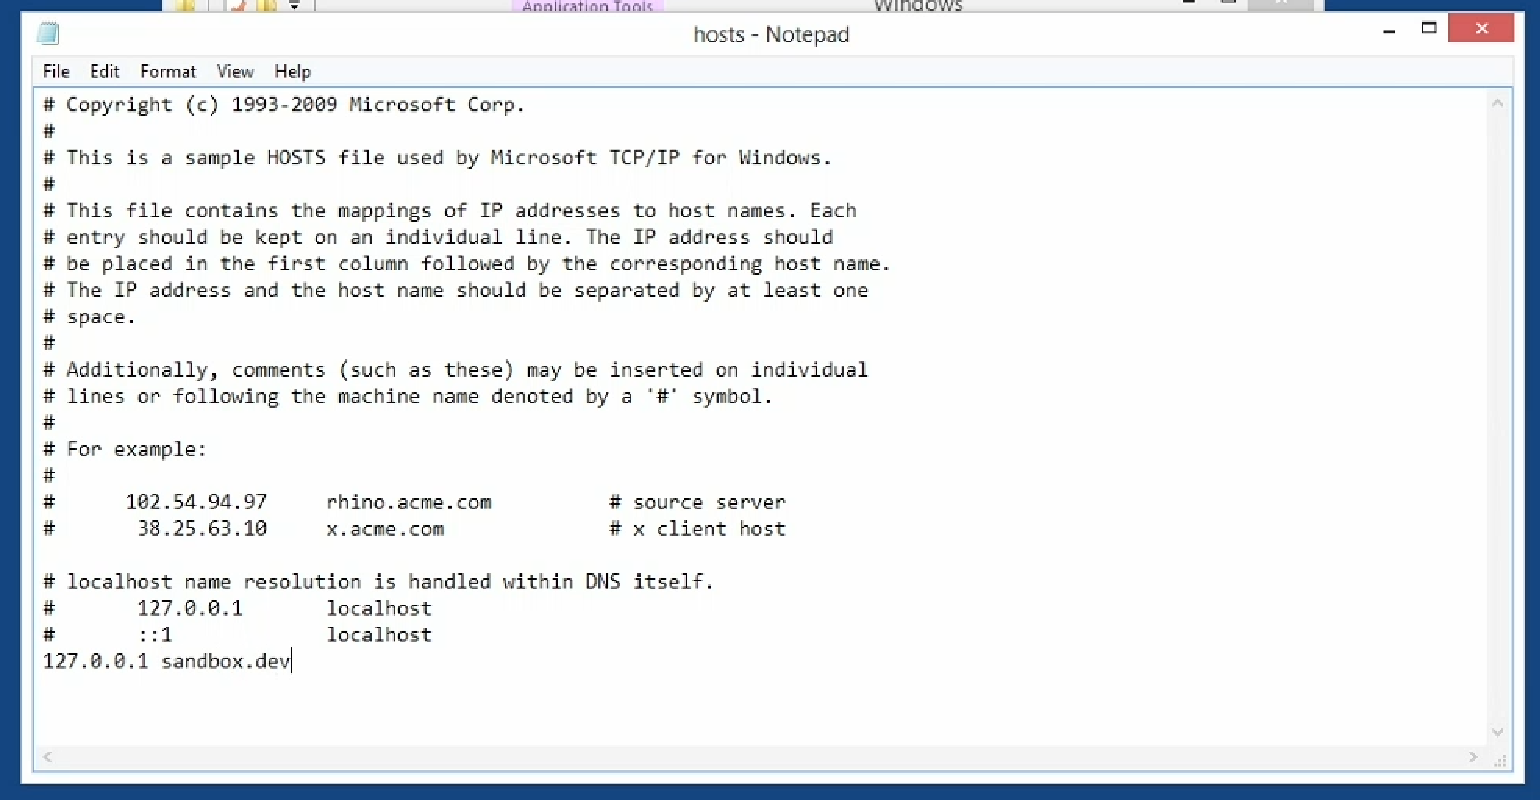
\includegraphics[width=.9\textwidth ,height=.55\textwidth]{Pic/WinHost}
    \caption{ پرونده تنظیم هاست در ویندوز 8}
    \label{win-hosts}
\end{figure}

\paragraph{استفاده از یک میزبان محلی مزایای زیر را دارد،}
\begin{itemize}
    \item
    سریع‌تر از یک میزبان اینترنتی بوده و به سرعت اینترنت شما بستگی ندارد.
    به اتصال به اینترنت و برخط بودن نیازی نیست و به صورت محلی می‌توانید برنامه خود را توسعه دهید.
    \item
    نیازی به خرید و مدیریت یک میزبان واقعی ندارید و به این ترتیب در هزینه‌ها صرفه جویی می‌شود.
    \item
    برای تست پایگاه وب خود نیازی به خرید یک دامنه اینترنتی منحصر به فرد و با معنی نخواهید داشت.
    
\end{itemize}

\part*{اتصال از طریق SSH}
\section{اتصال به سندباکس با استفاده از اس‌اس‌اچ «SSH»}
بعد ز آنکه توانستیم به سیستم بفهمانیم که 
\lr{sandbox.dev}
 را به آدرس آی‌پی 
\lr{127.0.0.1}
 نسبت دهد، وقت آن رسیده است که به نصب و تنظیم اس‌اس‌اچ بپردازیم. ما این ابزار را در هنگام نصب اوبونتو سرور نصب کرده‌ایم، بنا بر این نگرانی از این بابت نخواهیم داشت. اگر از گنو/لینوکس استفاده می‌کنید که باید این ابزار را توسط مدیر بسته‌های نرم‌افزاری خود نصب کنید.

\subparagraph*{نکته: }
پوشش تمامی این دستورات در توزیع‌های مختلف با روش‌های خاص خود کمی طولانی خواهد بود که از این موضوع صرف نظر می‌کنیم با این حال نصب آن بسیار آسان خواهد بود و حتی ممکن است در توزیع شما از پیش نصب باشد. در سیستم‌عامل او‌اس ده که به صورت پیش‌فرض نصب است.

همانطور که در ابتدای مطلب به آن اشاره داشتیم، ابزار اس‌اس‌اچ برای دسترسی به رایانه‌ای از راه دور کاربرد دارد. ما در این مورد قصد داریم تا با استفاده از سیستم خود سندباکس موجود در ویرچوال‌باکس را مدیریت کنیم. در فصل قبل و پیش از این، درگاه مورد نیاز این کار را به درگاه دلخواه 
\lr{2020}
 انتقال داده‌ایم که در قسمت قبل به طور مفصل به آموزش آن پرداختیم. پس برای دسترسی به سیستم مهمان می‌بایست از 
\lr{sandbox.dev}
 و درگاه شماره 
 \lr{2020}
  استفاده کنیم.

به دور وش می‌توان در اتصال به یک سیستم از راه دور از طریق اس‌اس‌اچ، هویت خود را احراز کنید. اولین گزینه این است که  از طریق نام کاربری و گذرواژه یکی از کاربران سیستم مقصد، هویتتان احراز شود و دومین روش با استفاده از یک کلید مشترک ایجاد شده است که باعث می‌شود تا مادامی که آن کلید را دارید، بدون نیاز به وارد کردن گذرواژه به سیستم مورد نظر دسترسی داشته باشید.

در سیستم‌عامل او‌اس ده اس‌اس‌اچ به راحتی قابل دسترسی است. فقط باید به ترمینال رفته و دستور را اجرا کنید. اما سیستم‌عامل ویندوز تنها سیستم‌عامل مطرح است که از اس‌اس‌اچ بی‌بهره است و برای نصب آن باید از ابزار PuTTY استفاده کرد. با این حال روش زیر نیز یکی از روش‌های نصب اس‌اس‌اچ در ویندوز است.

از پیوند مقابل  
\path{OpenSSH for Windows v3.8.1p1-1}
، این برنامه را بارگیری کنید که یک پیوند مستقیم است.
آن را از حالت فشرده خارج کرده که به صورت یک فایل آرشیو و فشرده است سپس باید فایل مقابل را که نصاب برنامه است را اجرا کنید، 
\path{«setupssh.exe»}
.
مسیر نصب برنامه را از مسیر پیش‌فرض به مسیر  
\path{“C:\OpenSSH”}
  تغییر دهید تا دسترسی به تنظیمات و … برایتان راحت باشد.
تنظیمات در شاخه بالا و در زیر شاخه 
\path{/etc}
 واقع شده‌اند.

گفتنی است خبرهایی مطرح شده است که امکان دارد در ویندوز ۱۰ از اس‌اس‌اچ به طور پیش‌فرض استفاده شود.

سپس بعد از انجام دادن کامل کارهای بالا، در هر یک از سیستم‌عامل‌ها خط فرمان را باز کنید و دستور زیر را وارد کنید.

\begin{latin}
    \lstinputlisting[numbers=right,language=SH, framexleftmargin=5mm, frame=shadowbox,rulesepcolor=\color{Black}]{Code/code4.sh}
\end{latin}

در دستور بالا شماره درگاه بعد از کلید 
\lr{«-p»}
 و نام‌کاربری قبل از نام دامنه سفارشی  نوشته شده است که با  واژه ات‌ساین  
\lr{«@»}
 از نام میزبان «sandbox.dev» جدا شده است. سپس پیغام زیر نمایش داده خواهد شد که برای تایید آن کلمه بله «yes» را از وارد کنید و سپس کلید اینتر را از صفحه‌کلید بفشارید تا پیغام بسته شود.
\\
\begin{latin}
    \lstinputlisting[numbers=right,language=SH, framexleftmargin=5mm, frame=shadowbox,rulesepcolor=\color{Gray}]{Code/code5.sh}
\end{latin}
سپس گذرواژه نام کاربری را وارد کرده و منتظر ورود به خط فرمان سیستم مهمان شوید. بعد از آن هر دستوری را که بخواهید می‌توانید در داخل اوبونتو اجرا کنید. کار بعدی ما این است که یک کلید خاص و مختص به خود  را برای استفاده ایجاد نماییم. این مورد را فقط یک بار انجام خواهید داد و دیگر نیازی به انجام آن در هر بار دسترسی نخواهید داشت. ابتدا دستور زیر را در خط فرمان اجرا کنید که هرچه در بین جفت کوتیشن درج شده است را به عنوان یک پیغام «کامنت» در نظر خواهد گرفت و کلید ایجاد شده نیز «rsa» خواهد بود.
\\
\begin{latin}
    \lstinputlisting[numbers=right,language=SH, framexleftmargin=5mm, frame=shadowbox,rulesepcolor=\color{Black}]{Code/code6.sh}
\end{latin}
سپس بعد از آن، از ما مکانی برای ذخیره شدن کلید درخواست می‌شود که پیش‌فرض گزینه‌ای مناسب است. در پیغام بعدی از شما درخواست می‌شود تا یک گذرواژه برای احراز هویت خود با این کلید انتخاب کنید. ما در سندباکس گذرواژه‌ای در نظر نمی‌گیریم. اما اگر خواستید می‌توانید برای رمز خود یک گذرواژه در نظر بگیرید. سپس کلید ساخته شده و در خروجی برای شما به نمایش در خواهد آمد.
\\
\begin{latin}
    \lstinputlisting[numbers=right,language=SH, framexleftmargin=5mm, frame=shadowbox,rulesepcolor=\color{Black}]{Code/code-rsa.txt}
\end{latin}
بعد از آن باید پوشه مخفی ssh. را در رایانه مجازی مهمان ایجاد کنید. برای این‌کار دستور اس‌اس‌اچ را به همراه دستور ساخت پوشه «mkdir» اجرا می‌کنیم. بعد از اجرای دستور زیر، اس‌اس‌اچ اجرا شده اما بعد از اجرای این دستور، اس‌اس‌اچ مجددا بسته خواهد شد.
\
\begin{latin}
    \lstinputlisting[numbers=right,language=SH, framexleftmargin=5mm, frame=shadowbox,rulesepcolor=\color{Black}]{Code/code7.sh}
\end{latin}
سپس ما کلید خصوص ایجاد شده توسط دستور  کَت «cat» را به کلیدهای احراز هویت در مقصد یعنی رایانه مهمان منتقل می‌کنیم. برای این کار دستور زیر را اجرا کنید که خروجی دستور کت را با دستور کت دیگر  به یک فایل در ماشین مهمان می‌ریزد.
\
\begin{latin}
    \lstinputlisting[numbers=right,language=SH, framexleftmargin=5mm, frame=shadowbox,rulesepcolor=\color{Black}]{Code/code8.sh}
\end{latin}
سپس بعد از اجرای دستور بالا، و نوشتن گذرواژه، فایل بالا در سیستم مهمان با محتوای کلید ایجاد شده توسط سیستم میزبان پر خواهد شد.  اگر دستور بالا برایتان مشکل است نگران نباشید، زیرا دستور بالا طولانی ترین دستوری بود که تا آخر این آموزش با آن مواجه خواهید شد. با وجود این دستور بالا با وجود طولانی بودن ساختار آسانی دارد. سپس بعد از انجام عملیات بالا، اگر بخواهید وارد سیستم مهمان شوید، دیگر نیازی به گذرواژه نخواهید داشت. 

البته اگر در هنگام ساخت کلید عمومی گذرواژه‌ای را در نظر گرفته بودید، باید آن گذرواژه را در هر بار اتصال به رایانه مجازی یا سیستم مهمان وارد کنید، زیرا کلید شما نیز خود نیاز به یک گذرواژه دارد. به همین دلیل پیشنهاد ما این بود که از گذرواژه در سندباکس استفاده نکنید، مگر آنکه به یک شبکه عمومی متصل باشید و از جهات امنیتی شبکه خود نگران هستید.
\\
\begin{latin}
    \lstinputlisting[numbers=right,language=SH, framexleftmargin=5mm, frame=shadowbox,rulesepcolor=\color{Black}]{Code/code9.sh}
\end{latin}
اگر دقت کرده باشید، هنگام نوشتن دستور بالا کمی خسته خواهید شد و حتماً باید شماره درگاه و نام کاربری را وارد کنید که در هربار اتصال یکسان است. حال که از نوشتن گذرواژه آسوده شدیم، بهتر است از موارد نیز  خود را برهانیم. در این هنگام با دستور خارج شدن «logout» از اس‌اس‌اچ خارج شوید و در سیستم میزبان دستور زیر را وارد کنید تا فایل مورد نظر برای انجام این کار ویرایش شود.
\\
\begin{latin}
    \lstinputlisting[numbers=right,language=SH, framexleftmargin=5mm, frame=shadowbox,rulesepcolor=\color{Black}]{Code/code10.sh}
\end{latin}
آنگاه بعد از باز شدن ویرایشگر متن نانو، متن زیر را وارد کنید و با کلید‌های Ctrl+X و نوشتن واژه «Y»، فایل را ذخیره کنید.
\\

\begin{latin}
    \lstinputlisting[numbers=right,language=SH, framexleftmargin=5mm, frame=shadowbox,rulesepcolor=\color{Black}]{Code/ssh-conf.txt}
\end{latin}

در ابتدای خط دوم و سوم یک بار کلید Tab را فشار دهید. بعد از آن با دستور زیر به راحتی به سیستم مهمان متصل خواهید شد.

\begin{latin}
    \lstinputlisting[numbers=right,language=SH, framexleftmargin=5mm, frame=shadowbox,rulesepcolor=\color{Black}]{Code/code11.sh}
\end{latin}
\section{ اتصال SSH در ویندوز:}
\paragraph*{    نکته: }
    اگر کاربر سیستم‌عامل‌های شبه یونیکس، او‌اس ده و گنو/لینوکس هستید این قسمت را مطالعه نکنید.
    
    . برای اتصال به سیستم مهمان از طریق اس‌اس‌اچ، ابتدا نرم‌افزار PuTTY را از  این پیوند دریافت و بارگیری کنید. سپس بعد از نصب برنامه بالا آن را از طریق منوی استارت اجرا کرده و در قسمت تنظیمات PuTTY موارد مورد نیاز و وارد شده در قسمت‌های قبلی را به صورتی که در تصویر  مشاهده می‌کنید، وارد کنید. و سپس بر روی دکمه Save کلیک کنید. \ref{PUTTY1}
\begin{figure}
    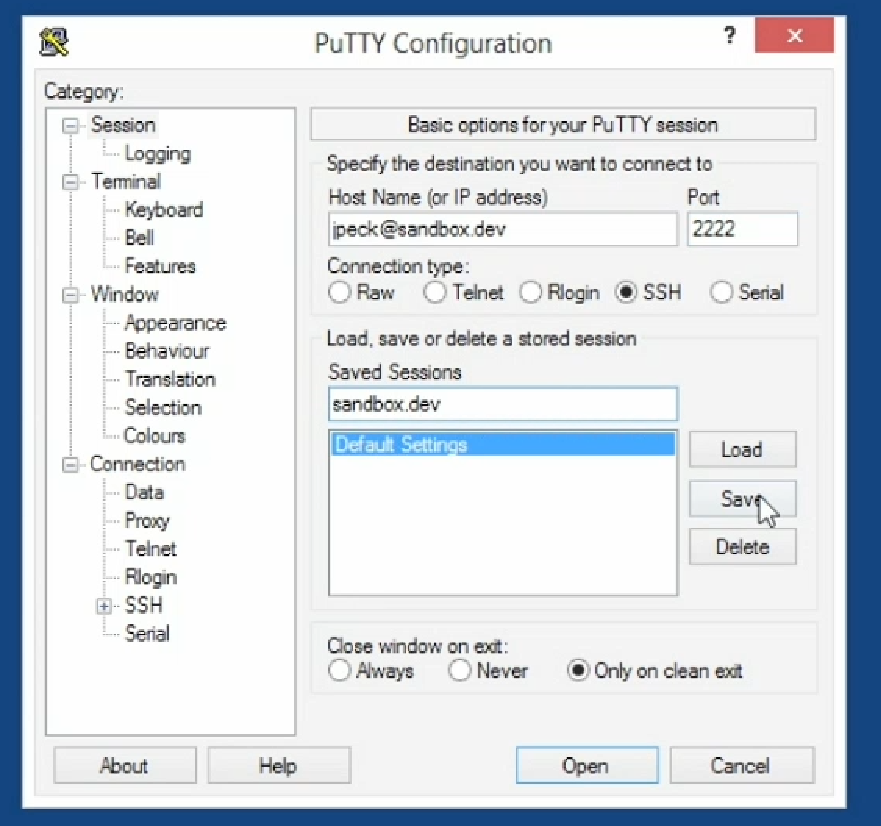
\includegraphics[width=.89\textwidth ,height=.85\textwidth]{Pic/PUTTY1}
    \caption{ نمایی از نرم افزار PUTTY}
    \label{PUTTY1}
\end{figure}

بعد از این کار با کلیک مضاعف بر روی نام سرور یعنی sandbox.dev، اتصال برقرار شده و خط فرمان باز خواهد شد. همانطور که مشاهده می‌شود پیغام خطایی نمایش داده می‌شود که برای اولین بار نمایش داده خواهد شد. بدون توجه به پیغام بالا که می‌گوید این سیستم ناشناخته است بر روی دکمه Yes کلیک کنید.  سپس گذرواژه از شما پرسیده می‌شود که با ورود آن می‌توانید وارد سیستم مهمان شوید. ممکن است در زمان نوشتن گذرواژه هیچ حرفی مشاهده نشود، این یک ایراد نیست بلکه یک مزیت است! بدون نگرانی گذرواژه را وارد کرده و کلید اینتر را بفشارید.

برای ایجاد یک کلید عمومی در ویندوز به منوی استارت رفته و برنامه PuTTY-Gen را اجرا کنید. سپس مطمئن شوید که گزینه SSH-2 RSA فعال باشد و سپس بر روی دکمه Generate کلیک کنید.  \ref{PUTTY2}
\\
\begin{figure}
    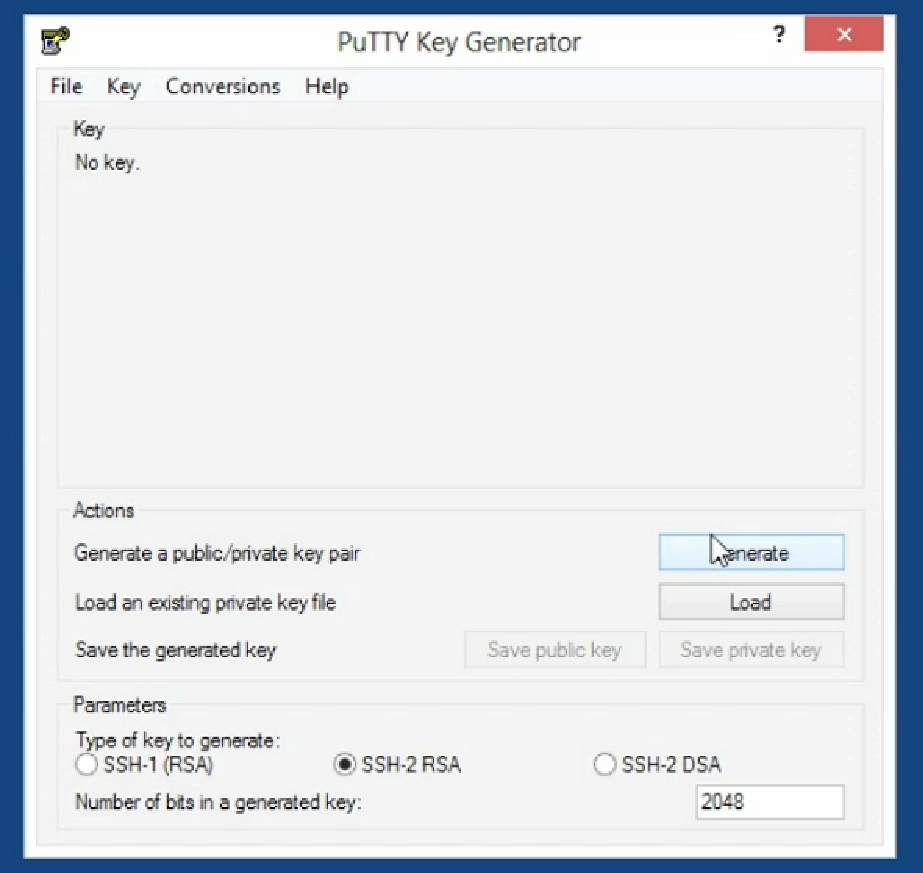
\includegraphics[width=.89\textwidth ,height=.85\textwidth]{Pic/PUTTY2}
    \caption{ نمایی از  تنظیمات   PUTTY}
    \label{PUTTY2}
   \end{figure} 
   
بعد از آن بقیه قسمت‌ها مانند کامنت «Comment»  و … را نیز پر کنید. در این قسمت آدرس رایانامه خود را وارد کنید. \ref{PUTTY2}

در مقابل کادر «Passphrase» می‌توان گذرواژه‌ای دلخواه را بنویسید. ما در سندباکس گذرواژه‌ای در نظر نمی‌گیریم. اما اگر خواستید می‌توانید برای رمز خود یک گذرواژه در نظر بگیرید. برای ذخیره کلید بر روی دکمه 
\lr{«Save private key»}
 کلیک کرده و مکان مناسبی را برای ذخیره آن در نظر بگیرید. به عنوان نمونه آن را در میزکار و با نام private ذخیره کنید. سپس هر آنچه در کادر بزرگ بالای پنجره ایجاد شده را کپی کرده و سپس مجدد PuTTY را اجرا کنید و با نوشتن گذرواژه وارد سیستم مهمان شوید. بعد از وارد شدن به سیستم مهمان دستورات زیر را در خط فرمان وارد کنید. 
\begin{latin}
    \lstinputlisting[numbers=right,language=SH, framexleftmargin=5mm, frame=shadowbox,rulesepcolor=\color{Black}]{Code/code12.sh}
\end{latin}
و بعد از آن دستور زیر را اجرا کنید، فقط به جای متن نوشته شده بین “” متن کپی شده از کادر بالا را جایگزین کنید.
\begin{latin}
    \lstinputlisting[numbers=right,language=SH, framexleftmargin=5mm, frame=shadowbox,rulesepcolor=\color{Black}]{Code/code13.sh}
\end{latin}
سپس هنگامی که از سیستم خارج شدید، کلید ذخیره شده در میزکار را اجرا کنید تا PAgent اجرا شود و در این هنگام اگر بخواهید مجدداً به وسیله PuTTY وارد سیستم مهمان شوید، دیگر نیازی به نوشتن گذرواژه نخواهید داشت.
\section{نصب چند نرم‌افزار مورد نیاز برای پیکربندی سندباکس}
برنامه‌ها در اوبونتو سرور با استفاده از خط فرمان و دستور ای‌پی‌تی «APT» انجام می‌شود. این ابزار می‌تواند لیست برنامه‌های نصب شده را با لیست موجود در اینترنت همگام کند و سپس بسته‌های نرم‌افزاری را بر اساس آن به روز کند. همچنین با این ابزار می‌توان نرم‌افزارها را نصب و حذف نمود. به طور کلی برای مدیریت بسته‌های نرم‌افزاری به کار می‌رود.

در ‎
\path{/etc/apt/sources.list}
آدرس منابع نرم‌افزار قرار گرفته‌اند. این منابع می‌توانند سی‌دی، دی‌وی‌دی، فایل تحت شبکه یا پوشه‌های اف‌تی‌پی یا اچ‌تی‌تی‌پی باشند. اگر بسته‌ای در پوشه‌ها یا دیسک سخت موجود باشد خودکار دریافت شده و نصب می‌گردد. تمامی بسته‌ها با فرمت دب (قالب پرونده) می‌باشند و پیش‌نیازها به صورت خودکار شناسایی شده‌اند، برای همین ممکن است در هنگام نصب برنامه‌ای کتابخانه‌های مورد نیاز هم دریافت و نصب گردند. نرم‌افزار ای‌پی‌تی یا اپت از روی دی‌پی‌کی‌جی کار می‌کند. 
\begin{flushleft}
    (ویکی‌پدیا، دانشنامه آزاد)
\end{flushleft}

ابتدا سیستم خود را با استفاده از ای‌پی‌تی به روز کنید. برای این کار ابتدا باید لیست نرم‌افزارهای موجود با لیست نرم‌افزار در سرور و ویرایش‌های به‌روز شده در آن همگام شود، سپس بعد از همگام شدن لیست با دستور به‌روزرسانی سیستم، هر نرم‌افزاری که ویرایش جدید از آن در دسترس است را نصب خواهد کرد، یعنی اگر ویرایش نرم‌افزار از ۱٫۰٫۱ به ۱٫۰٫۲ تغییر کرده است ویرایش جدید آن نرم‌افزار یعنی ویرایش جدیتر ۱٫۰٫۲ را به جای قبلی نصب و جایگزین خواهد کرد.
\begin{latin}
    \lstinputlisting[numbers=right,language=SH, framexleftmargin=5mm, frame=shadowbox,rulesepcolor=\color{Black}]{Code/code14.sh}
\end{latin}
بعد از نصب تمامی به‌روزرسانی‌ها حال باید ماشین مجازی را با دستور زیر راه‌اندازی مجد کنید. بعد از راه‌اندازی مجدد باید دوباره از طریق اس‌اس‌اچ به آن متصل شوید. فرآیند به‌روزرسانی حدود ۵ دقیقه از زمان شما را خواهد گرفت.
\begin{latin}
    \lstinputlisting[numbers=right,language=SH, framexleftmargin=5mm, frame=shadowbox,rulesepcolor=\color{Black}]{Code/code15.sh}
\end{latin}
اولین نرم‌افزاری که قرار است نصب کنیم، زی‌شل نام دارد که جایگزینی برای BASH به شمار می‌رود.  زی‌شل و تنظیمات و برخی ابزارهای مرتبط با آن را نصب می‌کنیم تا بتوانیم راحت‌تر دستورات را بنویسیم در این پوسته خط فرمان اگر چند حرف دستوری را بنویسید و کلید TAB را بفشارید، آن دستور را برای شما کامل خواهد کرد. به طور کلی سرعت شما را در نوشتن دستورات خط فرمان بلا خواهد برد.

امکانات آن از صفحه زی‌شل ویکی‌پدیا،
\begin{itemize}
    \item
مکمل خط فرمان قابل برنامه‌ریزی که می‌تواند به نوشتن آپشن‌ها و آرگومان‌ها برای بیشتر دستورها کمک کنند و دارای پشتیبانی از چند صد دستور بدون نیاز به تنظیم خاصی است.
\item
به اشتراک‌گذاری تاریخچه دستورها بین همه پوسته‌ها،
\item
الگوهای توسعه‌یافته‌ای که توصیف پرونده را بدون نیاز به برنامه‌ای خارجی مانند زدااچ «ZSH» است.
\item
متغیر/آرایه بهبودیافته،
\item
ویرایش دستورهای چندخطی در یک بافر،
\item
غلط‌یاب،
\item
حالت‌های سازگاری مختلف، برای مثال \textbf{zsh} می‌تواند به‌مانند 
\lr{Bourne shel}
l رفتار کند اگر به‌عنوان 
\path{‎/bin/sh}
 اجرا گردد.
\item
واسط خط فرمان قابل پوسته‌بندی، شامل توانایی قراردادن اطلاعات در سمت راست صفحه و داشتن آن به صورت مخفی به صورت خودکار مخفی هنگام نوشتن یک دستور طولانی،
\item
ماژول‌های قابل بارگیری، فراهم‌کنندهٔ قابلیت‌های از حمله: کنترل‌کنندهٔ TCP و 
\lr{Unix domain socket}
 کامل، یک کلاینت اف‌تی‌پی و توابع ریاضی توسعه‌یافته،
\item
کاملاً قابل تنظیم، 
\end{itemize} 
\begin{flushleft}
    ویکی‌پدیا ، دانشنامه آزاد
\end{flushleft}
برای نصب زی‌شل و دیگر ابزار مرتبط دستور زیر را اجرا کنید. در دستور تغییر شل «chsh» هنگام پرسیدن مسیر شل مورد نظر نیز همان مسیر نوشته شده در زیر را وارد کنید. ‘گفتنی است که اگر بخواهید برنامه‌ای را نیز توسط ای‌پی‌تی نصب نماید در هنگام نوشتن نام بسته‌ها اگر چند حرف از آن را بنویسید و کلید «TAB» را بزنید، نام نرم‌افزارها کامل خواهد شد.
\begin{latin}
    \lstinputlisting[numbers=right,language=SH, framexleftmargin=5mm, frame=shadowbox,rulesepcolor=\color{Black}]{Code/code16.sh}
\end{latin}
بعد از اجرای دستور بالا، در خط فرمان با نوشتن زی‌شل به شکل لاتین «zsh» شل مذکور را اجرا کرده و در سوالی که پرسیده می‌شود، عدد 0 را تایپ کرده و کلید اینتر را از صفحه کلید فشار دهید. سپس تمامی نرم‌افزارهای مورد نیاز برای موارد بعدی در آینده را نصب خواهیم کرد. برای این کار دستور زیر را اجرا کنید.
\begin{latin}
    \lstinputlisting[numbers=right,language=SH, framexleftmargin=5mm, frame=shadowbox,rulesepcolor=\color{Black}]{Code/code17.sh}
\end{latin}

\section{اتصال پوشه اشتراکی در ویرچوال‌باکس}
بعد از نصب ابزار مورد نیاز نوبت به اتصال پوشه اشتراک گذاشته شده در ویرچوال‌باکس می‌شود. برای این‌کار شما باید پوشه‌ای با نام Sandbox را در جایی در سیستم میزبان ایجاد کنید. سپس از طریق روش اشاره شده در قسمت اول آن را با ویرچوال‌باکس در سیستم مهمان به اشتراک بگذارید. بعد از آن اگر تیک اتصال خودکار فعال باشد در هر بار اجرای سیستم آن پوشه برای سیستم شناخته شده خواهد بود. پوشه بالا در شاخه 
\path{media/sf_sandbox/}
  اتصال یافته است. اما در اوبونتو سرور برای دسترسی کامل به آن پوشه باید راه‌انداز و ابزار اضافی ویرچوال‌باکس در اوبونتو نصب شود که شامل موارد متعددی است. برای نصب آن از منوی Devices گزینه 
  \lr{Insert Guest Additions CD image}
   را انتخاب کنید تا تصویر این ابزار در سیستم مهمان به عنوان دیسک مجازی شناخته ‌شود. \ref{VBox5}
  \\
  \begin{figure}
      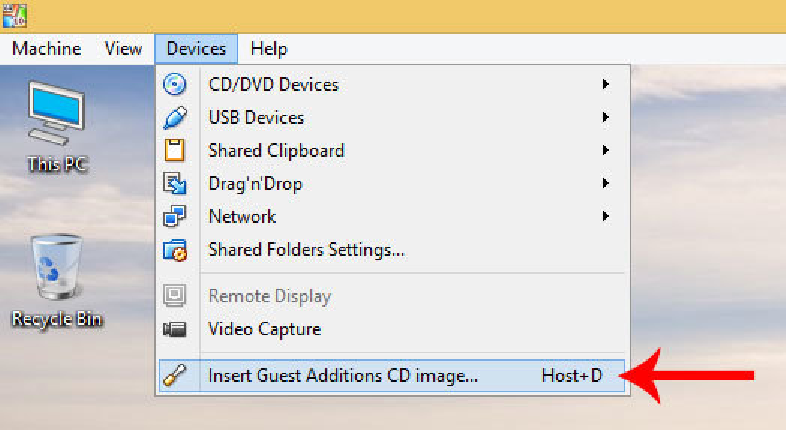
\includegraphics[width=.89\textwidth ,height=.45\textwidth]{Pic/VBox5}
      \caption{ تصویر راه انداز ویرچوال باکس}
      \label{VBox5}
    \end{figure} 
بعد از انجام عمل بالا، می بایست که دیسک را نیز به پوشه‌ای در شاخه مدیا 
\path{/media}
 متصل کنید، برای این کار باید دستور 
\lr{Mount}
 را به شکل زیر استفاده کنید.
\begin{latin}
    \lstinputlisting[numbers=right,language=SH, framexleftmargin=5mm, frame=shadowbox,rulesepcolor=\color{Black}]{Code/code18.sh}
\end{latin}
اگر پیغامی نمایش داده شد نگران نشوید زیرا مرتبط با این موضوع است که دیسک بالا به صورت فقط خواندنی است. سپس دستور زیر را برای نصب این ابزار در گنو/لینوکس در ترمینال سیستم مهمان  وارد کنید.
\begin{latin}
    \lstinputlisting[numbers=right,language=SH, framexleftmargin=5mm, frame=shadowbox,rulesepcolor=\color{Black}]{Code/code19.txt}
\end{latin}
اخطار آخر برای این نمایش داده شده است که در اوبونتو سرور ابزار گرافیکی برای نمایش پنجره‌ها و … که کارساز  نمایشگر 
 \lr{X.Org}
  نام دارد نصب نیست که نیازی به این ابزار هم وجود ندارد. سپس ماشین مجازی را مجددا راه‌اندازی مجدد کنید. (طبق دستوراتی که در نوشته‌های قبلی ذکر شد.) حال اگر دستور زیر را اجرا کنید، خواهید فهمید که ماژول‌های مورد نظر در اوبونتو به خوبی بالا آمده‌اند. ماژول‌های بالا با کلمه 
  \lr{«vbox»}
   آغاز شده‌اند.
\newline
\begin{latin}
    \lstinputlisting[numbers=right,language=SH, framexleftmargin=5mm, frame=shadowbox,rulesepcolor=\color{Black}]{Code/code20.txt}
\end{latin}
برای دسترسی به پوشه اشتراکی باید به مسیر 
\path{media/sf_sandbox/}
 بروید.
 
\begin{latin}
    \lstinputlisting[numbers=right,language=SH, framexleftmargin=5mm, frame=shadowbox,rulesepcolor=\color{Black}]{Code/code21.sh}
\end{latin}
که همانطور که می‌بینید با پیغام خطای عدم اجازه برای دسترسی مواجه خواهید شد. برای اینکه بتوانید به این  مجوز لازم را به کاربر جاری یعنی خودتان بدهید باید خودتان را برای دسترسی به آن مجاز کنید. ابتدا بیایید بررسی کنیم این فایل چه مجوز دسترسی خاصی دارد.

\begin{latin}
    \lstinputlisting[numbers=right,language=SH, framexleftmargin=5mm, frame=shadowbox,rulesepcolor=\color{Black}]{Code/code22.sh}
\end{latin}
این فایل برای کاربرانی که عضو گروه 
\lr{vboxsf}
 هستند مجاز است. حال بیایید ببینیم آیا ما در این گروه عضو هستیم یا خیر، برای این‌کار دستور زیر را اجرا کنید تا تمامی گروه‌هایی که شما در آنان عضو هستید را نمایش دهد.


\begin{latin}
    \lstinputlisting[numbers=right,language=SH, framexleftmargin=5mm, frame=shadowbox,rulesepcolor=\color{Black}]{Code/code23.sh}
\end{latin}
شما در گروه‌های زیادی عضو هستید. این گروه‌ها یک مشخصه خاصی نیز به همراه خود دارند. اگر به این لیست دقت کنید، هیچ یک از این گروه‌ها 
\lr{vboxsf}
 نیستند. پس کدام حساب کاربری در این گروه عضو است؟ برای فهم این موضوع دستور زیر را اجرا کنید.

\begin{latin}
    \lstinputlisting[numbers=right,language=SH, framexleftmargin=5mm, frame=shadowbox,rulesepcolor=\color{Black}]{Code/code24.sh}
\end{latin}

در دستور بالا با استفاده از ابزار 
\lr{getent}
 و مشخص کردن نام گروه و جستجوی گروه‌ها در بانک‌اطلاعاتی گروه‌های کاربری، مشاهده می‌شود که هیچ کاربر خاصی در این گروه حضور ندارد. پس چاره‌ای نمی‌ماند جز اینکه با دستور زیر حساب کاربری خود را به عضویت این گروه در‌آورید.  دستور مورد استفاده دستور 
 \lr{usermod}
  خواهد بود. برای اجرای دستور بالا نیز مانند دستورات سیستمی مورد استفاده در موارد قبلی باید از 
\lr{sudo}
   استفاده کنیم تا دسترسی بیشتری داشته باشیم.

\begin{latin}
    \lstinputlisting[numbers=right,language=SH, framexleftmargin=5mm, frame=shadowbox,rulesepcolor=\color{Black}]{Code/code25.sh}
\end{latin}
با وجود این اگر یک‌بار از حساب خود خارج و مجدد وارد حساب خود نشوید، قادر نیستید که به این پوشه دسترسی یابید. برای اعمال تغییرات کاربری و افزودن و حذف از گروهی خاص، باید یک‌بار از حساب خود خارج شوید و سپس وارد حساب کاربری خود شوید. همچنین بعد از انجام تغییرات بالا، دقت داشته باشید که آپاچی نیز قرار است به این پوشه دسترسی داشته باشد. برای اینکه بتواند محتوای آن را نمایش دهد، باید حساب کاربری  
\lr{www-data}
نیز بتواند به این پوشه اجازه دسترسی داشته باشد. خوب اگر دستور زیر نیز اجرا شود این دسترسی تخصیص خواهد یافت که این دستور مطابق دستور بالا عمل کرده با این تفاوت که به جای نام کاربری خود نام کاربری \lr{www-data} جایگزین شده است.
\begin{latin}
    \lstinputlisting[numbers=right,language=SH, framexleftmargin=5mm, frame=shadowbox,rulesepcolor=\color{Black}]{Code/code26.sh}
\end{latin}

\part*{راه اندازی ابتدایی کارساز}
\section{تنظیم و پیکربندی آپاچی}
آپاچی یک کارساز وب متن‌باز و آزاد است که توسط بنیاد آپاچی توسعه‌داده می‌شود، اطلاعات بیشتر در این مورد را می‌توانید در قسمت اول این مقاله مطالعه کنید. اکثر فایل‌های پیکربندی نرم‌افزارها و ابزار در گنو/لینوکس در شاخه  
\path{/etc}
 قرار دارد. اگر به پوشه مخصوص تنظیمات آپاچی واقع در پوشه apache2 در شاخه 
\path{/etc}
 بروید،پوشه‌های زیر را در آن خواهید دید. \ref{code27}
\newline
\begin{latin}
    \label{code27}
    \lstinputlisting[numbers=right,language=SH, framexleftmargin=5mm, frame=shadowbox,rulesepcolor=\color{Black}]{Code/code27.txt}
\end{latin}

برای ان که آپاچی به درگاه و آدرس مورد نظر ما پاسخ دهد باید در تنظیماتی که در 
\lr{sites-available}
 هستند را به پوشه 
\lr{site-enabled}
 منتقل کنید، اما اکثرا این کار را با ایجاد یک میانبر از پوشه در دسترسها به پوشه فعالها انجام می‌دهیم. اگر به داخل پوشه تنظیمات 
\lr{sites-available}
 بنگریم تنظیمات پیش‌فرض را مشاهده خواهیم کرد. ما به این تنظیمات نیازی نداریم. بنابراین تنظیمات خود را با استفاده از نانو 
 \lr{"ٔNANO"}
  ایجاد می‌کنیم، اگر بدون تنظیمات خاصی آپاچی را اجرا کنید، با صفحه بالا مواجه می‌شوید. \ref{UbuntuServer-Apache}

\begin{figure}
    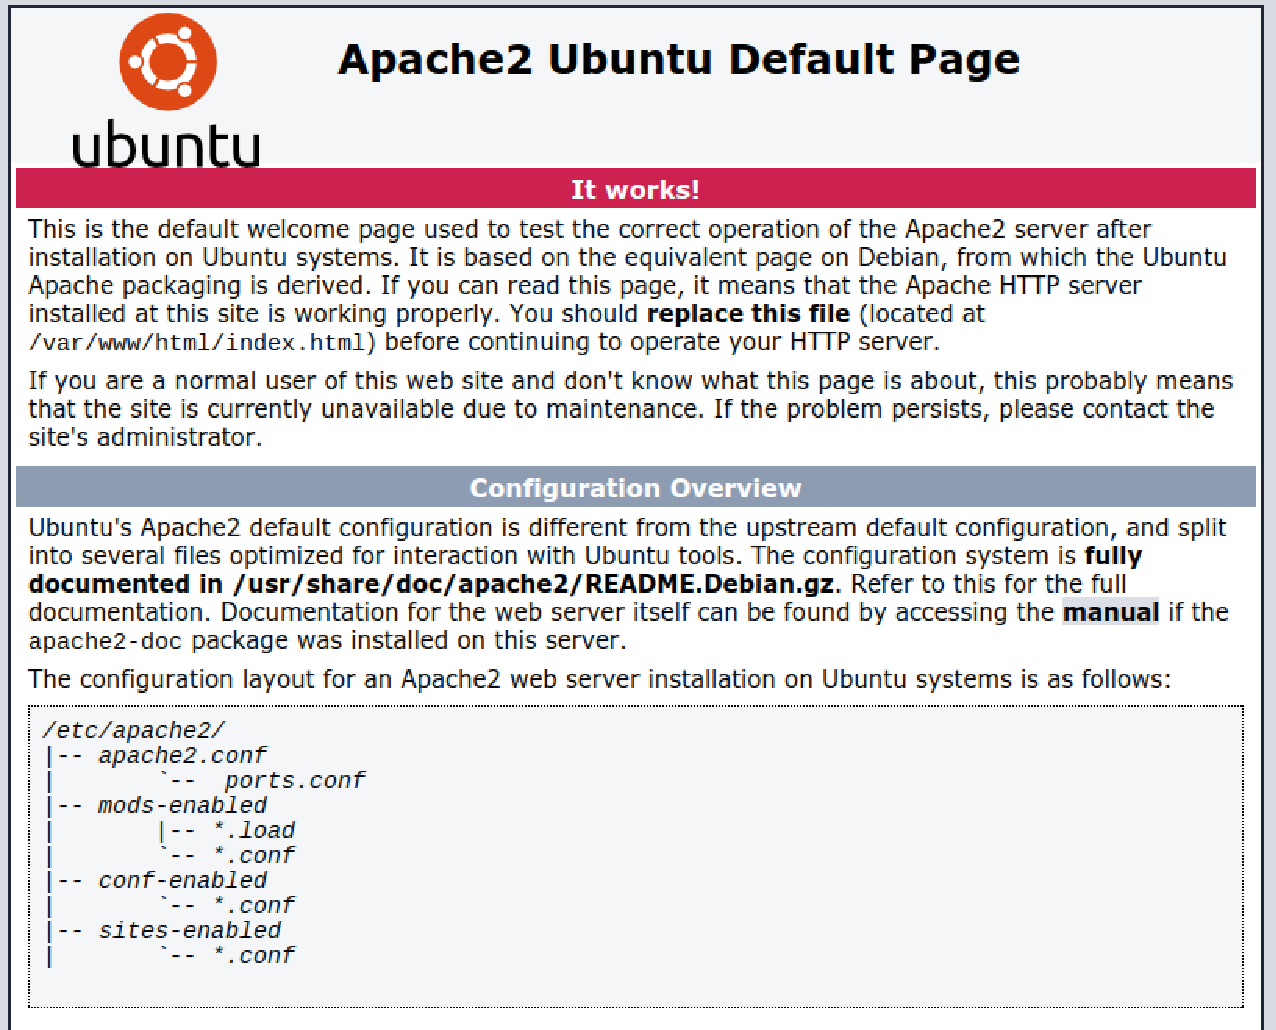
\includegraphics[width=.9\textwidth ,height=.65\textwidth]{Pic/UbuntuServer5}
    \caption{ نمایی از  آپاچی هنگامی که تنظیم نشده است}
    \label{UbuntuServer-Apache}
\end{figure}
\subsubsection{ویرایش فایل‌ها توسط sudoedit}
یکی از دستوراتی که برای ویرایش فایل‌های سیستمی به کار می‌رود دستور sudoedit است که ابتدا یک کپی از فایل در شاخه موقتی 
\path{/tmp}
 کپی کرده و بعد از ویرایش کامل روی همان فایل می‌ریزد. این ویرایشگر از ویرایشگر نانو استفاده می‌کند. با استفاده از این ویرایشگر متنی فایل تنظیمات مورد نیاز خود را برای اجرای سرور و کارساز وب آپاچی ایجاد می‌کنیم.
\newline
\begin{latin}

    \lstinputlisting[numbers=right,language=SH, framexleftmargin=5mm, frame=shadowbox,rulesepcolor=\color{Black}]{Code/code27.sh}
\end{latin}
در داخل آن محتویات زیر را نوشته و سپس فایل را ذخیره می‌کنیم.
\newline
\begin{latin}
   
    \lstinputlisting[numbers=right,language=SH, framexleftmargin=5mm, frame=shadowbox,rulesepcolor=\color{Black}]{Code/VBox.conf.txt}
\end{latin}
سپس باید آن درگاهی را که از مهمان به میزبان منتقل کرده‌ایم و آن را به 
\lr{8080}
 تغییر داده‌ایم را به کارساز وب آپاچی بشناسانیم. برای این کار باید از دستور زیر استفاده کرد که فایل را ویرایش کرده و تنظیمات مورد نیاز را در آن وارد می‌کنیم.
\newline
\begin{latin}
    
    \lstinputlisting[numbers=right,language=SH, framexleftmargin=5mm, frame=shadowbox,rulesepcolor=\color{Black}]{Code/code28.sh}
\end{latin}

در آن فایل بعد از کلمه 
\lr{Listen 80} 
و خط بعدی باید
\lr{Listen 8080}
 را وارد کرد.  بعد از آن فایل بالا باید مشابه زیر باشد.
\newline
\begin{latin}
    
    \lstinputlisting[numbers=right,language=Bash, framexleftmargin=5mm, frame=shadowbox,rulesepcolor=\color{Black}]{Code/ports.conf.txt}
\end{latin}
با استفاده از دستورات 
\lr{«a2ensite»}
 و 
\lr{«a2dissite»} 
 میتوانید سایتی را فعال و یا غیر فعال کنید، این دستورات میانبری از فایل تنظیمات مورد نظر در «sites-available» در داخل پوشه «sites-enabled» ایجاد خواهد کرد. برای فعال کردن تنظیماتی که خودمان وارد کردیم، باید با استفاده از دستورات بالا آنان را فعال کنیم، برای این کار باید دستور زیر را اجرا کنیم.
\newline
\begin{latin}
    
    \lstinputlisting[numbers=right,language=Bash, framexleftmargin=5mm, frame=shadowbox,rulesepcolor=\color{Black}]{Code/code29.sh}
\end{latin}
دستورات 
\lr{a2dissite}
 را نیز برای غیر فعال کردن تنظیمات پیش‌فرض به کار می‌گیریم.
\begin{latin}
    
    \lstinputlisting[numbers=right,language=Bash, framexleftmargin=5mm, frame=shadowbox,rulesepcolor=\color{Black}]{Code/code30.sh}
\end{latin}
همچنین تا زمانیکه برخی ماژول‌ها را فعال نکرده‌اید، آپاچی را نمی‌توانید اجرا کنید. زیرا با خطا مواجه خواهید شد. برای فعال یا غیر فعال کردن ماژول در آپاچی ۲ از دستورات 
\lr{«a2enmod»}
 و 
\lr{«a2dismod»}
  استفاده می‌شود. با استفاده از دستور زیر ماژول 
\lr{«rewrite»}
   را فعال می‌کنیم.
\begin{latin}
    
    \lstinputlisting[numbers=right,language=Bash, framexleftmargin=5mm, frame=shadowbox,rulesepcolor=\color{Black}]{Code/code31.sh}
\end{latin}
ماژول‌های بعدی که باید فعال شوند، ماژول‌های 
\path{«vhost_alias»}
 و 
\path{ «status»}
  هستند که این ماژول‌ها را نیز با دستور زیر می‌توانید فعال کنید.
\begin{latin}
    
    \lstinputlisting[numbers=right,language=Bash, framexleftmargin=5mm, frame=shadowbox,rulesepcolor=\color{Black}]{Code/code32.sh}
\end{latin}

بعد از آنکه با موفقیت توانستید تمامی ماژول‌های بالا را فعال کنید،  قادر خواهید بود تا آپاچی را مجددا راه‌اندازی کنید و سرویس بالا را از نو اجرا کنید. این کار در هر بار تنظیم آپاچی باید صورت گیرد.
\begin{latin}
    
    \lstinputlisting[numbers=right,language=Bash, framexleftmargin=5mm, frame=shadowbox,rulesepcolor=\color{Black}]{Code/code33.sh}
\end{latin}
بعد از انجام تمامی مراحل بالا و برای آزمودن تنظیم بودن آپاچی ۲ و همچنین آزمودن صحت تنظیمات انجام شده در بالا، فایلی با نام 
\lr{«phpinfo.php»}
 را در پوشه 
 \lr{ «Sandbox» }
 (پوشه‌ای است مورد استفاده در ویرچوال‌باکس، برای اشتراک گزاری در ماشین مجازی) ایجاد کنید و مقادیر زیر را در آن وارد کنید.
\newline
\begin{latin}
    \lstinputlisting[numbers=right,language=PHP, framexleftmargin=5mm, frame=shadowbox,rulesepcolor=\color{Black}]{Code/phpinfo.php}
\end{latin}

\begin{figure}
    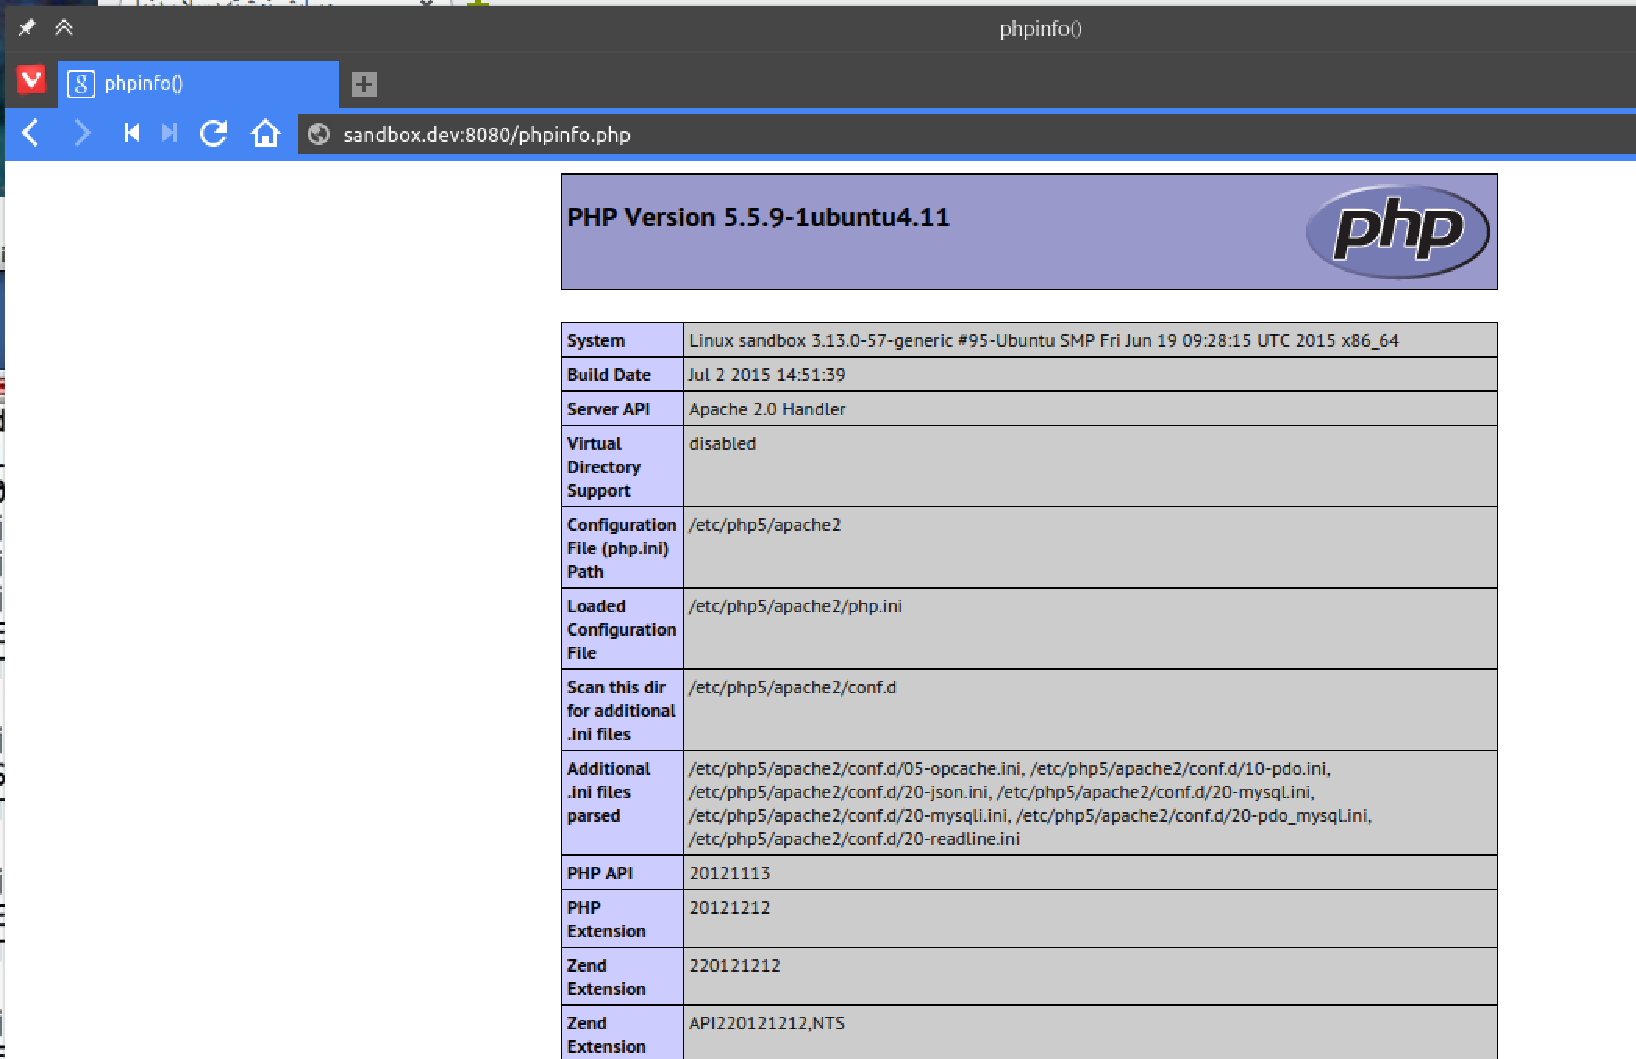
\includegraphics[width=.9\textwidth ,height=.65\textwidth]{Pic/PHPINFO}
    \caption{ نمایی از 
        \lr{phpmyinfo()}
        هنگامی که  آپاچی و 
        \lr{PHP}
         تنظیم شده است}
    \label{PHPINFO}
\end{figure}
سپس در مرورگر آدرس زیر را وارد کنید تا صفحه‌ای مشابه تصویر را مشاهده کنید. اگر همه‌چیز به خوبی اجرا شد و صفحه مشابهی را مشاهده کردید، تنظیمات به خوبی انجام شده و آپاچی به درستی در حال کار است. \ref{PHPINFO}
\begin{latin}
\url{http://sandbox.dev:8080/phpinfo.php}
\end{latin}
در این فصل به تنظیم آپاچی و اتصال به سندباکس از طریق اس‌اس‌اچ پرداختیم. در فصل  بعدی کتاب عنی قسمت سوم این آموزش به تنظیمات نهایی و نصب برخی ابزارها و نرم‌افزارهای مورد نیاز خواهیم رسید که برای یک توسعه‌دهنده وب مورد نیاز هستند. تا اینجای کار قادر خواهید بود  که اکثر کارهایی قابل انجام در یک کارساز وب را انجام دهید، با وجود این برخی نکات کاربردی دیگر نیز وجود دارند که در قسمت بعدی به موارد بیشتری اشاره خواهم کرد.